\documentclass[12pt,a4paper]{article}
\usepackage{graphicx}
\usepackage{xcolor}
\usepackage[margin=0.8in]{geometry}
\usepackage{titling}
\usepackage{indentfirst}
\usepackage{wrapfig}
\usepackage{amsfonts}
\usepackage{tocloft}
\usepackage{tabularx}
\usepackage{listings}
\renewcommand{\cftsecleader}{\cftdotfill{\cftdotsep}}
\setlength{\parindent}{0em}




\title{\textbf{CAOS Projekt : 2 x 6 x 12 LED RGB Quader}}
\author{Joey Zgraggen, Moritz Würth, Viktor Gsteiger}

\begin{document}
\renewcommand\contentsname{Inhaltsverzeichnis}
\begin{titlepage}
\maketitle
TODO: BILD VOM PROJEKTERZEUGNIS
\end{titlepage}
\tableofcontents
\newpage

\section{Einführung}

Die Grundidee von unserem Projekt war es zuerst einen 5 x 5 x 5 LED RGB Würfel zu bauen, jedoch haben wir uns dann im Prozess der Entscheidungsfindung
dazu entschieden, etwas anderes zu bauen was sich vom "typischen" LED RGB Würfel unterscheidet.
Deshalb haben wir die Dimensionen ein wenig angepasst, sodass wir am Ende einen dreidimenstionalen Bildschirm haben werden. Damit wird es uns immer noch möglich sein, gute 3D-Effekte
anzeigen zu können. Die Anordnung der LED's kann als Koordinatensystem verstanden werden, bei dem man mittels x- und y-Koordinaten auf die einzelnen LED's zugreifen kann. Dies erleichtert es massiv, Effekte zu schreiben. 
Das Projekt lässt einen grossen Spielraum bezüglich Ideen zu. Sollte man also selbst Ideen haben, welche sich gut zu unserem Projekt ergänzen würden, kann man diese ohne weitere
Probleme implementieren. Die Grundsoftware hat sehr einfache Schnittstellen, mit denen man einfach weitere Effekte schreiben kann.


\section{Verwendete Materialien}

Im Folgenden ist eine Auflistung der verschiedenen Materialien, welche für das Projekt verwendet wurden.

\subsection{RGB LED's}

Um den LED-Quader ein wenig bunter gestalten zu können wurden RGB's verwendet.:

\begin{itemize}
    \item LED RGB Common Cathode 4-Pin F5 5MM Diode
\end{itemize}

\subsection{Schieberegister}

Schieberegister erweisen sich für ein solches Projekt als äusserst nützlich, um die vielen Pins der einzelnen RGB LED's ansprechen zu können. \\

Wir haben uns dabei an schon bereits existierende Projekte orientiert und uns für die 74HC595 8-bit Schieberegister entschieden. Diese erweisen sich in der Programmierung als intuitiv, weil man einfach mit Byte-Arrays arbeiten kann, um die einzelnen Schieberegister mit Informationen zu "befüllen". Weiter existieren für diese Schieberegister vorgefertigte Libraries, um die Kommunikation zu erleichtern.
Dies nimmt einen nicht die Denkarbeit ab, wie man die LED's anordnen will und wie man die verschiedenen Farben anspricht, jedoch erleichtert es die direkte Kommunikation.

\subsection{\textcolor{red}{Transistoren}}

Anfangs wollten wir für eine garantierte Langlebigkeit unseres Projektes Transistoren verwenden, aber nachdem wir uns bezüglich der Notwendigkeit
von Transistoren für unser Projekt informierten haben wir uns letzenendlich dazu entschieden keine zu verwenden.

\subsection{Sensoren}

Für das Projekt wurden zusätzlich Sensoren verwendet, um weitere Features zu gewährleisten. Diese werden im Kapitel 6 detaillierter behandelt.

Folgende Sensoren stehen zur Auswahl:
\begin{itemize}
    \item Temperatur und Luftfeuchtigkeitssensor
    \item Infrarot-Sensor
    \item Real-time clock
\end{itemize}

%\section{Materialkosten}
%
%\begin{tabularx}{\textwidth}{p{0.25\textwidth} | l | l | l | r |}
%    \textbf{Produkt} & \textbf{Menge} & \textbf{Preis} & \textbf{Total} \\
%    % Viktor's Ausgaben:
%    \cline{1-4}
%    RGB LED's & 250x & 0.072.- & 18.- \\
%    \cline{1-4}
%    Kabel (verschiedene) & 15m & 0.83.- & 12.50 \\
%    \cline{1-4}
%    Wiederstände & 440x & 0.036.- & 16.- \\
%    \cline{1-4}
%    74hc595 & 57x & 0.50.- & 30.- \\   
%    \cline{1-4}
%    Sensoren (verschiedene) & 3x & 3.30.- & 10.- \\
%    \cline{1-4}
%    Lochrasterplatine (verschiedene) & 2x & 6.00.- & 12.- \\
%    	% Total Viktor: 98.5.-
%    \cline{1-4}
%    Kupferdraht (Blau) & 2 Rollen & 6.80.- & 13.60.- \\
%    \cline{1-4}
%    Isolierband & 1 Rolle & 1.80.- & 1.80.- \\
%    \cline{1-4}
%    &&&\textbf{113.90.-}
	% Joey's Ausgaben: 20.0.-
	% Moritz's Ausgaben: 40.0.-
    
%\end{tabularx}

\section{Hintergrund}

Nachdem wir viele Projekte im Internet gefunden haben, welche unserem Projekt sehr nahe kommen, 
hat dies bei uns die Motivation erweckt, ebenfalls ein ähnliches Projekt zu machen.
Wir haben uns sehr intensiv in einem vorhandenen \textcolor{blue}{online Protokoll}\footnote{https://www.instructables.com/id/Arduino-Mega-8x8x8-RGB-LED-Cube/} bezüglich dem Bauen eines 
8x8x8 Quaders eingelesen, um Informationen zu sammeln, wie man das auf unser Projekt anweden könnte,
was für den Start unseres Projektes sehr hilfreich war. \\
Wir haben uns auch überlegt eine Box zu bauen, welche die ganze Lötarbeit in einem Raum verstaucht, um das ganze optisch ein wenig
angenehmer zu gestalten. Die verwendete Plexiglasscheibe ist mit Absicht durchsichtig, sodass man trotzdem noch
die damit verbundene Arbeit ansehen kann.





\section{Implementation}

Wie schon bereits erwähnt, haben wir uns nach schon bereits existierenden Projekten von RGB LED Cubes orientiert und konnten
auch anhand der vorhandenen Codes herausfinden, wie wir das Softwareseitig für unser Projekt am besten lösen können.
Für uns war das eine sehr grosse Hilfe, um dem Code eine gewisse Grundstruktur geben zu können. \\
Damit wir dem Code einen besseren Überblick verschaffen konnten und damit sich auch alle Gruppenmitglieder besser mit dem Code
auseinander setzen können haben wir den Code so unterteilt, dass die verschiedenen Bereiche wie Logik, Features und 
main separiert sind. \\\\
Unser verwendetes Konzept erlaubt es auch aussenstehenden Personen, welche am Projekt nicht teilgenommen haben und mit dem Code nicht sehr
vertraut sind ein eigenes Feature leicht zu implementieren und das Projekt zu erweitern. \\\\
Im Folgenden werden verschiedene von uns implementierten Feautes kurz erläutert.

\subsection{Alphabet}

Durch die Klasse Alphabet ist es einfach möglich, auf dem Bildschirm Buchstaben und Sätze darzustellen. Die Klasse unterscheidet nicht zwischen klein und Grossbuchstaben und kann das gesamte Alphabet plus ein paar Sonderzeichen plus alle Zahlen darstellen. Die einzelnen Buchstaben sind alle Hardgecoded und deshalb macht diese Klasse Sinn, weil man dies sonst jeweils einzeln machen müsste. Die Klasse Alphabet wird vom Willkommens Effekt, von den tempereature effects und vom clock Effekt benutzt und ist dadurch ein sehr zentraler Effekt.

Die Buchstaben werden dabei von rechts nach links einer nach dem anderen in den Buchstaben-Buffer geladen, dann jeweils, sofern man nicht beim letzten Buchstaben ist, drei mal auf den Hauptbildschirm rausgeshiftet und nach jedem einzelnen shiften angezeigt. Beim letzten Buchstaben wird dieser so lange nach links geshiftet, bis er vom Bildschirm verschwindet und die Kontrolle wird zurück an die rufer Methode gegeben.

\subsection{Stars}

Im Effekt stars werden zufällig Sterne erzeugt, welche entweder von links nach rechts oder umgekehrt fliegen. Wenn sich zwei Sterne treffen explodieren diese in einem Effekt. Die Sterne haben alle verschiedene Farben, welche auch zufällig sind. 

Die Sterne sind alle eigene structs, welche die nötigen Informationen beihnalten. In der Update methode werden alle existierenden Sterne fortgeführt in ihrem Pfad.

\subsection{Firework}

Der Feuerwerk Effekt funktioniert ähnlich wie der Sternen-Effekt, jedoch fliegen hier die Raketen nur von unten nach oben und explodieren auf einer zufälligen Höhe. Die Farbe der Raketen ist auch zufällig.

Eine Rakete ist ein struct, welche alle nötigen Informationen beinhaltet.

\subsection{Welcome}

Der Willkommens Effekt ist ein sehr einfacher Effekt, welcher einfach mit der Methode Alphabet eine Willkommensnachricht auf dem Bildschirm anzeigt und einmal nach dem Aufstarten angezeigt wird.

\subsection{Game of Life}

Der Game of Life Effekt ist eine repräsentation des berühmten Game of Life des britischen Mathematikers John Horton Conway. Dabei kommen  zufällig Zellen zum Leben und sterben beziehungsweise pflanzen sich nach bestimmten Regeln fort. Dabei können sie auch über den Bildschirmrand einen Effekt haben und zählen dann zu den Nachbaren auf der anderen Seite. Für mehr Informationen empfielt es sich, den Wikipedia Artikel zum Game of Life zu lesen.
§
\subsection{Snake}

Hierbei geht es um das klassische Snake Spiel, welches die meisten sicherlich schon kennen.
Man spielt eine Schlange (Snake), welche man in vier Richtungen mittels einer Infarot-Fernbedienung steuern kann.
Ziel ist es die verschiedenen "Pixel" (grün leuchtender RGB LED) zu erreichen, um damit die Schlange zu vergrössern.
Da die Implementation einige Probleme mit sich brachte, das Spiel so zu implementieren wie es eigentlich funktioniert, kann
man bei unserem Snake spiel sich selbst durchdringen. Das Spiel wird dadurch logischerweise etwas einfach, aber es ist trotzdem lustig
das Spiel mal auf eine andere Weise zu spielen.
Sollte man sich in die in die Wand (Rand) bewegen, dann ist das Spiel vorbei und man muss von vorne beginnen.

\section{Sensoren}

\subsubsection{Temperatur- und Luftfeuchtigkeitssensor}

Der Temperatur- und Luftfeuchtigkeitssensor, welchen wir für unser Projekt verwenden ist vom Typ DHT11. Dies ist ein eher einfacher Sensor, welcher jedoch mehr als genügt für unsere Zwecke. Dieser liest die aktuelle Temperatur und Luftfeuchtigkeit jede Sekunde und diese Information wird dann auf dem Bildschirm angezeigt. Mit Hilfe dieser Informationen wird dann aus einem von drei Effekten ausgewählt. Entweder wird dann ein Regen, Wolken oder eine Sonne auf dem zweidimensionalen Bildschirm angezeigt. Die Berechnung hierfür ist jedoch sehr einfach und rudimentär, weshalb der Bildschirm sich nicht für eine genaue Wettervorhersage eignet. 

\subsubsection{Infrarot-sensor}

Der Infrarot-sensor empfäng Input von einer externen Fernbedienung und man kann damit zwischen den verschiedenen Effekten wechseln. Dabei werden bei allen Effekten regelmässig die Informationen vom Sensor abgefragt und dann wird dies abgearbeitet. Wir haben uns hierbei extra gegen einen Interrupt gesteuerten Dateninput entschieden, weil dies das Effekthandling erschweren würde. So ist maximal ein Effekt zur gleichen Zeit am laufen und bricht ab, sobald man mit der Fernbedienung einen anderen Effekt auswählt.

Weiter kann man mit der Fernbedienung das Snake Spiel steuern und so die längste Schlange kreieren.

\section{Aufbau des zweidimensionalen Bildschirmes}

\subsection{Bildschirm}

\subsection{Schieberegister}

Wir bereits angesprochen helfen uns die Schieberegister die vielen verschiedenen Pins der RGB LED's anzusprechen.
Die Schieberegister sind auf zwei Platinen angeordnet und sind mit einander mittels den entsprechenden outputs miteinander
verknüpft. Wichtig war es dabei zu beachten, dass der Daten in- und output korrekt verlötet wurden, weil wir die Teilaufgaben
unseres Projektes untereinander aufgeteilt haben und die Anordnung der Schieberegister mit dem Code übereinstimmen müssen.

\subsection{Probleme beim Aufbau}

Durch die anspruchsvolle Steuerung von 216 einzelnen Pins kommt es
natürlich zu Schwierigkeiten. Unsere erste Schwierigkeit war, dass wir 
zuerst mit einer zu kleinen und einzelnen Platine gearbeitet haben. 
Dies hatte zur Folge, dass die Lötarbeit schnell unübersichtlich und ungenau wurde.
Auch war es so extrem schwer, die Lötstellen sauber zu verlöten. Wir haben uns nach einigem herumprobieren dafür entschieden, von einer auf zwei Platinen umzusteigen, was die Arbeit massiv vereinfacht hat.

\newpage
\section{Ergebnisse}

Im Folgenden ist der Prozess von unserem Projekt veranschaulicht: \\\\

Damit wir sichergehen konnten, dass alle gekauften Materialien in einem guten Zustand sind, haben wir diese erstmal 
getestet. Es wäre mühsam gewesen ein Schieberegister oder RGB LED nach Fertigstellung des Projektes auszutauschen: \\\\
\includegraphics[width=0.45\textwidth]{CAOSProject3.jpg}
\includegraphics[width=0.45\textwidth]{CAOSProject5.jpg} \\

Wie bereits erwähnt haben wir uns am Anfang dazu entschieden eine Platine für all unsere Schieberegister zu verwenden 
und haben dann im Verlaufe des Projektes bemerkt, dass das am Schluss sehr viel Aufwand mit sich bringt alle Kabel gut
auseinanderhalten zu können: \\\\
\includegraphics[width=0.45\textwidth]{CAOSProject7.jpg}
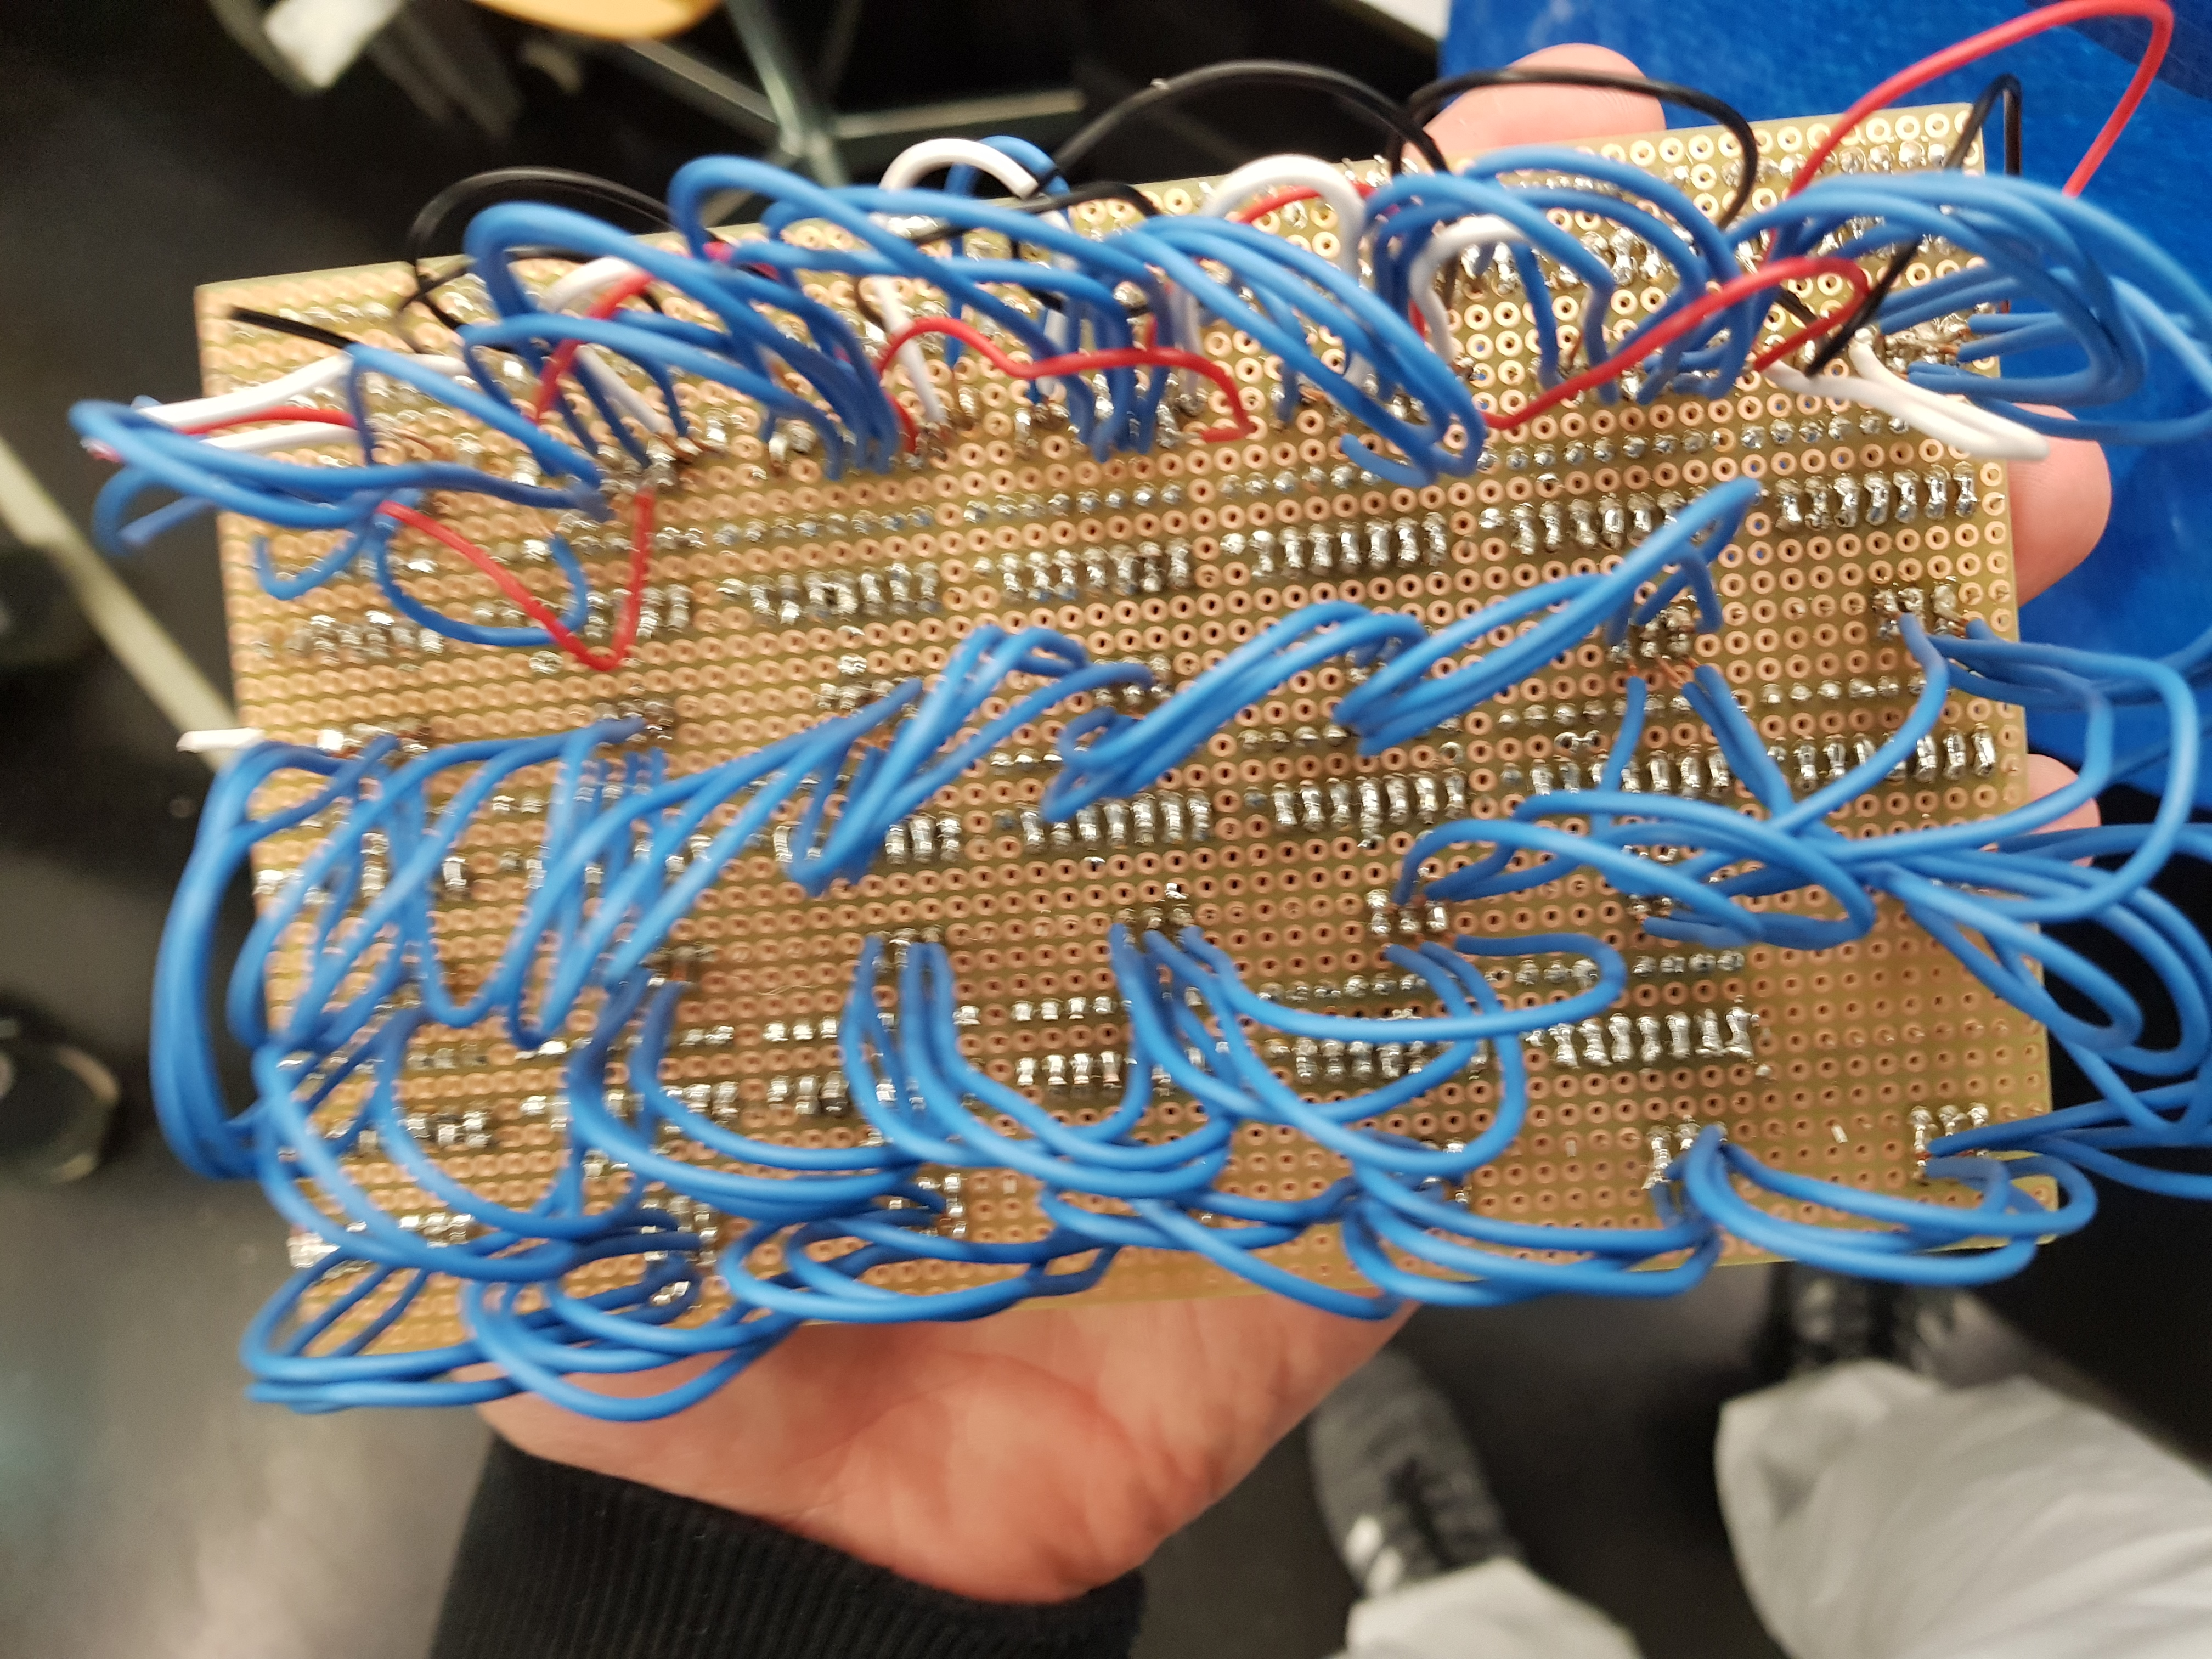
\includegraphics[width=0.45\textwidth]{CAOSProject8.jpg} \\\\
\newpage

Danach haben wir zwei Platinen verwendet, wodurch das Arbeiten um einiges erleichtert wurde: \\\\
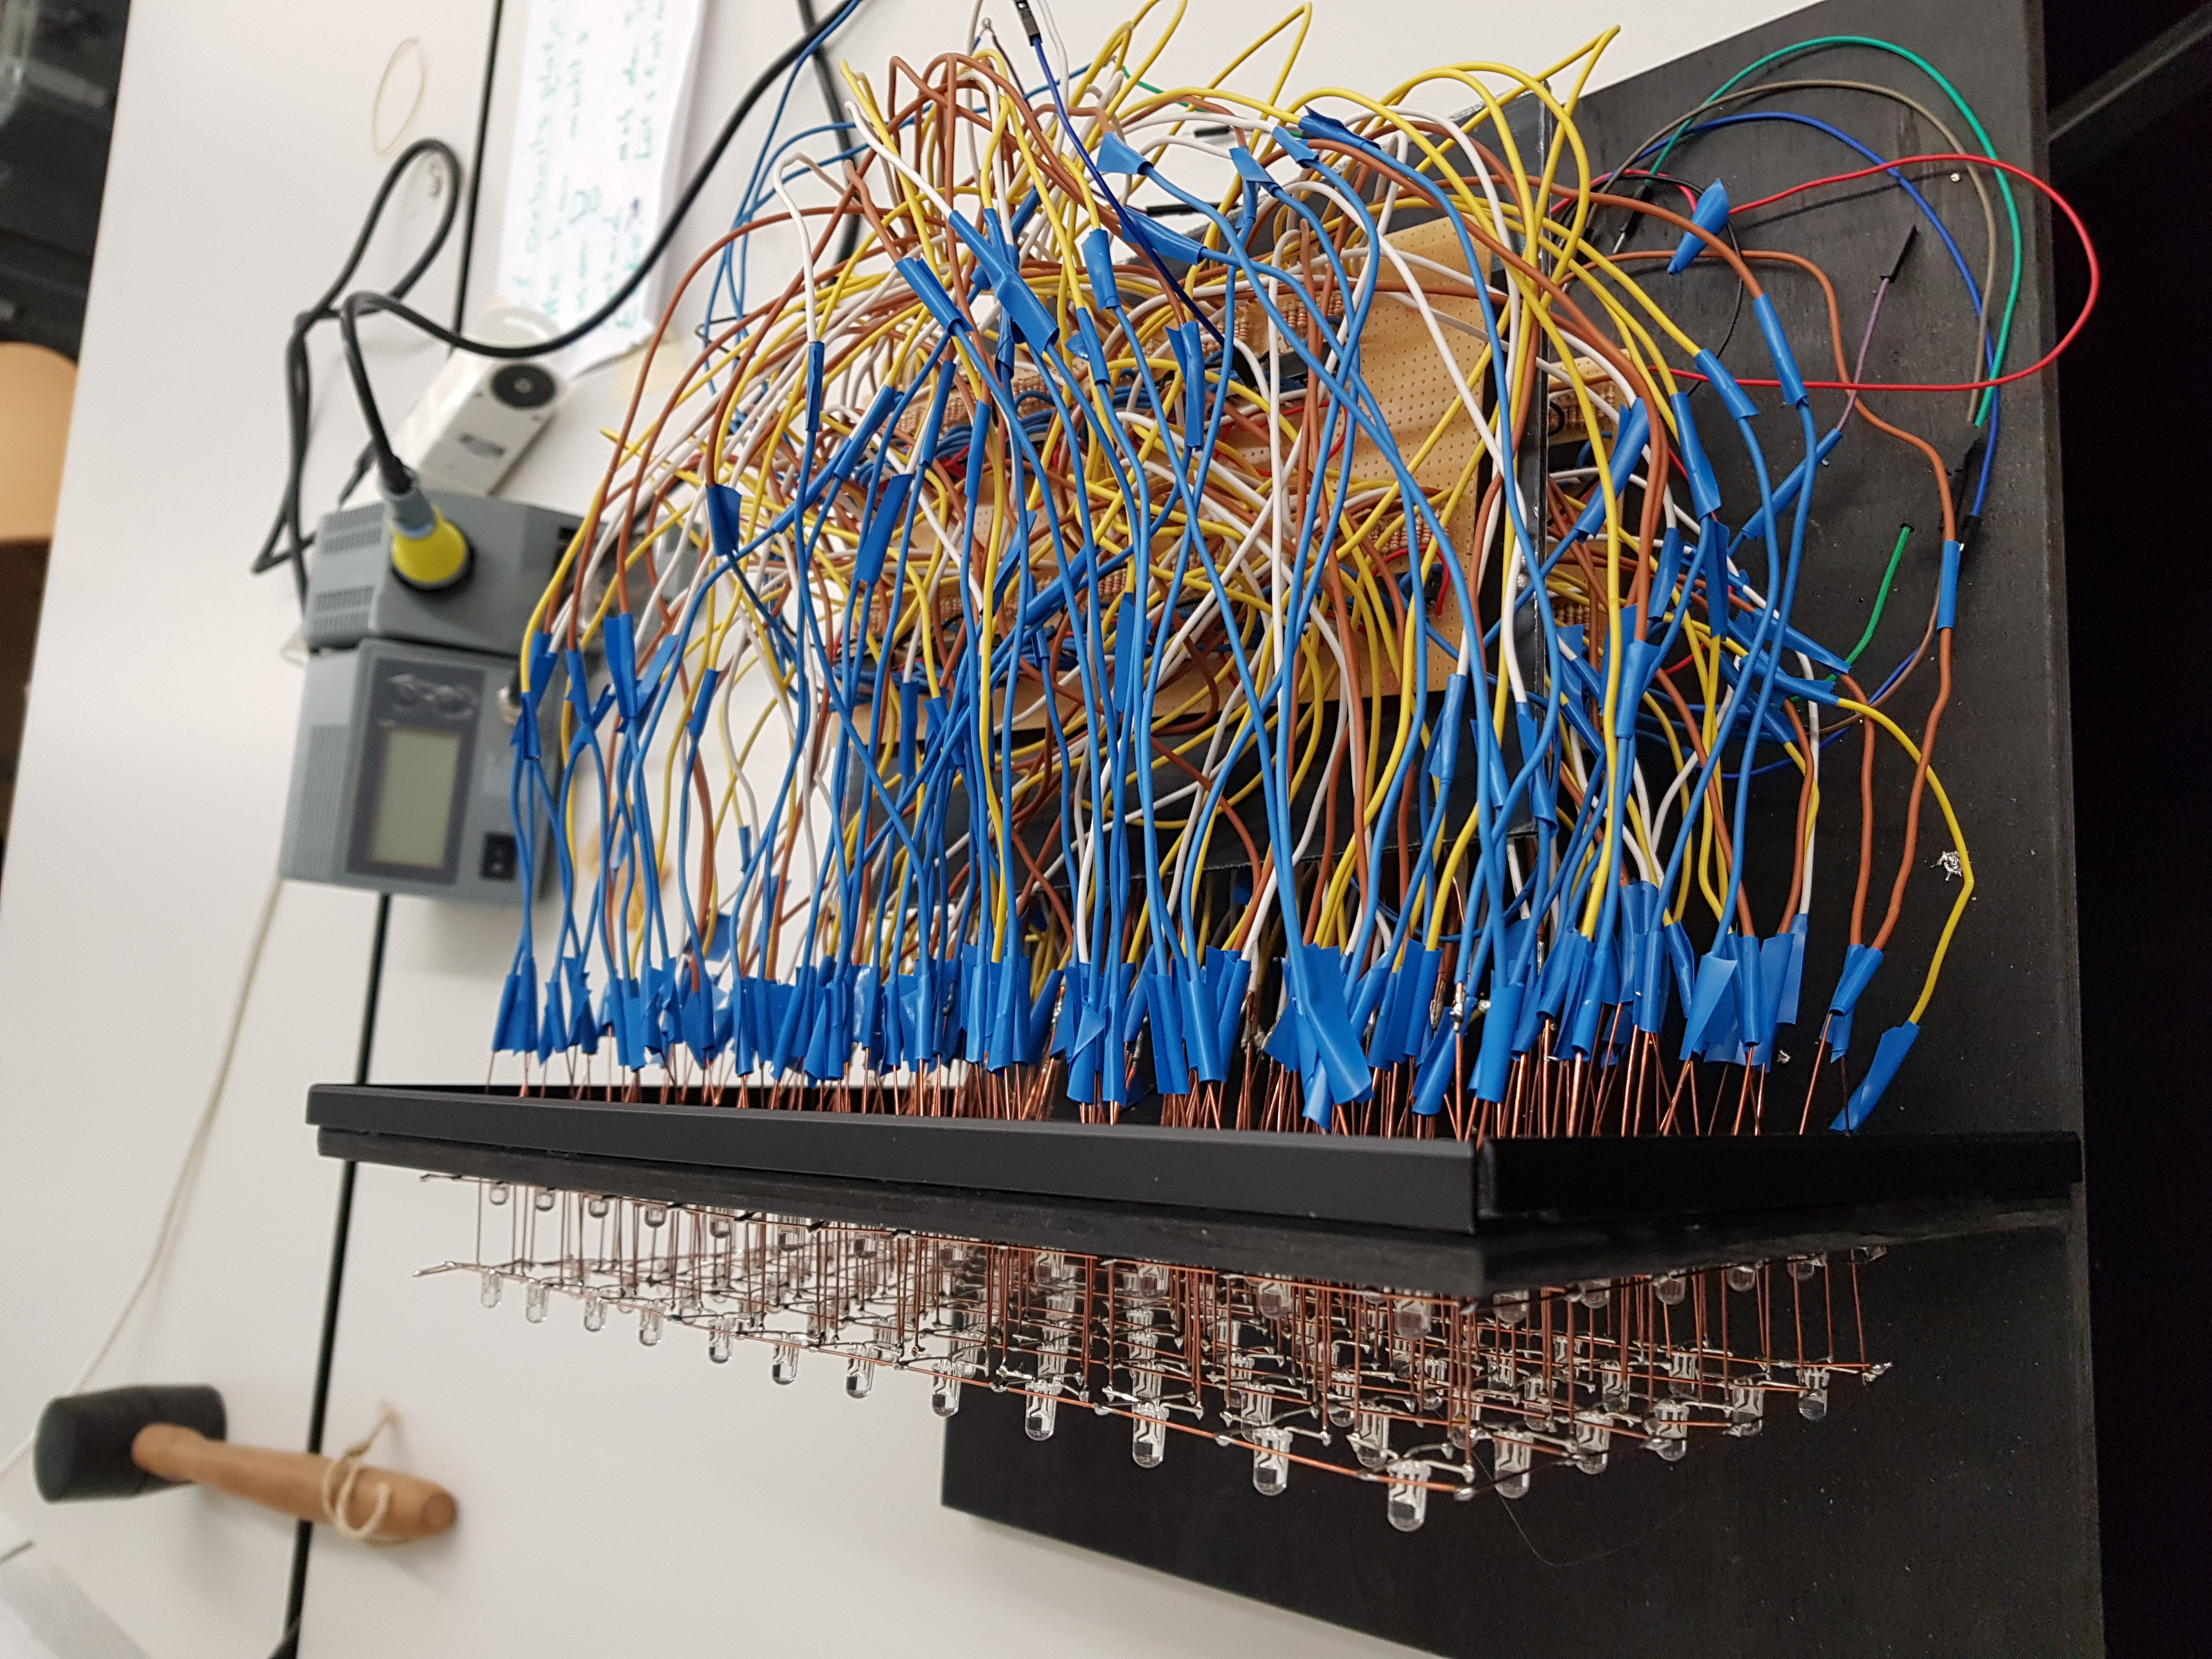
\includegraphics[width=0.45\textwidth]{CAOSProject9.jpg} \\\\

Am Schluss haben wir noch wie bereits erwähnt eine Verschalung aus Plexiglas (durchsichtig) gebaut, 
damit das ganze optisch besser aussieht: \\\\
\includegraphics[width=0.45\textwidth]{Endprod2.jpg}


\section{Zusammenfassung}

Da wir uns innerhalb der Gruppe schon sehr gut kennen und auch schon öfters zusammen gearbeitet haben, sei es in einem Projekt oder 
innerhalb der Übungsaufgaben war es für uns sehr angenehm, uns untereinander zu organisieren. Wir sind uns immer schnell einig gewesen,
beispielsweise zwei statt eine Platine zu verwenden, um die ganze Lötarbeit ein wenig effizienter zu gestalten, damit Parallel gearbeitet werden kann und
der ganze Hardware Teil unseres Projektes ein wenig übersichtlicher erscheinen zu lassen. \\\\
Auch wenn die Arbeit innerhalb der Gruppe in Hardware und Software unterteilt wurde, so haben wir doch immer wieder 
mal kleine Austausche durchgeführt, sodass jeder von beiden Bereichen erfolgreich etwas mitnehmen kann und die Zusammenhänge 
besser verstehen kann.
Jedes Gruppenmitglied hat mit dem Projekt neben der Vorlesung vie dazugelernt und es war eine sehr gute Erfahrung die groben Ansätze
der verschiedenen Themen der Vorlesung mit der Projektarbeit zu vertiefen.


\newpage

\textbf{Quellen}:

\begin{itemize}
    \item https://www.instructables.com/id/Arduino-Mega-8x8x8-RGB-LED-Cube/
    \item https://github.com/vGsteiger/caos\_gruppe\_144
\end{itemize}










\end{document}